\section{Introduction\label{sec:intro}}

%\begin{figure}[!htbp]
%    \centering
%    \includegraphics[height=5cm]{fig/1.pdf}
%    \caption{The distribution of the number of the graphical passwords.}
%\end{figure}

Pattern lock is widely used on Android devices to protect sensitive information. It is preferred by some users over PIN- or text-based
passwords, as psychology studies show that the human brain remembers and
recalls visual information better than numbers and
letters~\cite{DeAngeli:2005:PRW:1090412.1090419}.
According to a recent study, 40\% of the Android users
use patterns to protect their devices instead of a PIN~\cite{androidstudy}.
Pattern lock is also used for authentication. For example, \texttt{Alipay}, the largest
third-party online-payment platform, uses pattern lock for login authentication.
Given its pervasive usage, a security breach of the pattern lock could lead to serious consequences.


Researchers have demonstrated a number of ways to crack Android pattern lock.
For example, smudge attacks use the oily residues  left on the screen to recover
the pattern~\cite{aviv2010smudge}. However, this approach relies on the persistence of
the smudge which can be easily destroyed by subsequent on-screen activities after unlocking. In a recent study, Zhang
\emph{et al.}~\cite{zhang2016privacy} shows that it is possible to infer a locking pattern by analyzing how the WiFi signal is affected by the finger motions when drawing the pattern. Their approach is restricted to
a limit set of scenarios due two reasons: (1) the complex setup of the attacking environment and (2) the WiFi signal can be disrupted by any moving
objects nearby or body movements.


Recently, video-based side-channel attacks are shown to be effective in reconstructing PIN- or
text-based passwords. Some of the early work in this area rely on video
footage filmed using a camera directly facing the screen or the keyboard~\cite{
kuhn2002compromising, balzarotti2008clearshot}. Latest work shows that
this limit can be lifted by exploiting spatial-temporal dynamics of
the hands during typing~\cite{shukla2014beware}.
Despite the success of
video-based attacks on PIN- and text-based passwords, no work so far has
exploited video-based side-channels to crack pattern lock.
To do so, the attack must address a number of new challenges. These include: How to map the user's fingertip
movements to a graphical structure consisting of continuous points instead of discrete
keystrokes? How to transform the fingertip movements tracked from
the camera's perspective to the user's view point to correctly reconstruct the
pattern? How to cancel the camera shake effect that can significantly
affect the performance of the attack? how to identify two overlapping line segments
of a pattern? The size of the touch-screen or the pattern grid
can vary from one device or one application to the other, how can the algorithm
adapt to these changes?
These new challenges make prior work video-based attacks inapplicable.
To overcome these challenges requires creative
solutions to be constructed in the new application context of pattern lock.

%This is fundamentally
%different from a PIN or a text-based password consisting of discrete
%characters. Therefore, those techniques proposed in prior research on PIN-
%and text-based password attacks is not directly applicable to extract lock
%patterns from video footage.

%\FIXED{Considering its widely usage, pattern lock has already attracted
%attacker's attention. Researchers have proposed some attacks on Android
%pattern lock~\cite{aviv2010smudge,zhang2016privacy}. Among these attacks,
%Adam proposes a smudge attack by filming the image that contains the residual
%smudges after drawing the pattern lock~\cite{aviv2010smudge}. Such method,
%however, have a strong assumption that the attacker need to have the
%possession of the device for full controlling the lighting and camera
%condition to extract the smudgy information of pattern lock. Zhang proposes
%an attacking approach that can snoop the pattern lock by leveraging the
%impact of finer movement on the Wi-Fi signal while drawing the
%pattern~\cite{zhang2016privacy}. However, such approach is limited to the
%complex scenarios as other moving objects will greatly
%disturb the excepted Wi-Fi signal, making this approach perform poor in practical scenarios.}

%Computer vision based attacks have emerged as a new way of attacking
%text-based passwords on touched screen systems. \FIXED{Prior works have} made use of
%reflection of objects to reconstruct what the user types on the touched
%screen to recover the
%password~\cite{kuhn2002compromising,xu2013seeing,raguram2011ispy,backes2009tempest}.
%The previous methods relies on the use of a digital single-lens reflex (DSLR)
%camera to film the content of user input (e.g., chats, username, passwords),
%making this kind of attack easy to be found. Shukla et al. leverage the
%spatio-temporal dynamic of the hands to infer the pin based passwords
%\cite{shukla2014beware}. Similarly, Yue et al. identify the pin based
%passwords by light diffusion surrounding touched keys \cite{yue2014blind}.
%However, such attacking schemes need to know the layout of the keyboard (such
%as the size of each key and the location of each key on the keypad). Such
%assumptions, however, do not hold for pattern hock, making the prior work
%infeasible for attacking
%pattern-based lock.

This paper presents a novel approach to crack Android pattern lock using
video footage that captures the user's fingertip motions when drawing the pattern. Unlike smudge attacks~\cite{aviv2010smudge}, our approach
does not require the video footage or images to be captured by a camera
directly faced the screen. Furthermore, the video can be filmed at a
distance of 2 meters from the user in public places. Such a distance is less likely
to raise suspicion compared to shoulder
surfing~\cite{shoulder} that requires a
closer observation distance to have a clear sight of the content displayed on the screen. %This makes our attack is more likely to success
%when compared to previous attacks on pattern lock.

Our attack employs a computer vision algorithm to
track the fingertip motions from the video. Using the geometry
information extracted from the fingertip motions, it then maps
the tracked fingertip locations to a small number of (often just one)
candidate patterns to be tested on the target device.


   \begin{figure}[!h]
        \centering
        \subfigure{
            \begin{minipage}[t]{3.5cm}
            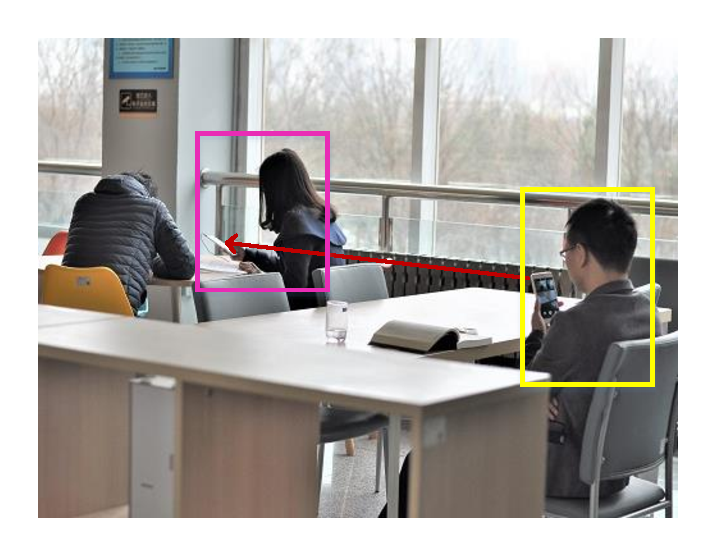
\includegraphics[height=3cm]{fig/1-1.pdf}\\
             \footnotesize (a) The user was listening to music and unaware of what was happening around.
            \end{minipage}
        }
        \hspace{0.5cm}
        \subfigure{
            \begin{minipage}[t]{3.5cm}
            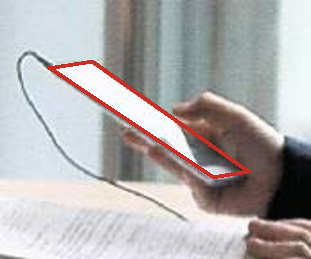
\includegraphics[height=3cm]{fig/1-2.pdf}\\
             \footnotesize (b) The device screen seen from the video filmed in (a).
            \end{minipage}
        }
        \subfigure{
            \begin{minipage}[t]{3.5cm}
            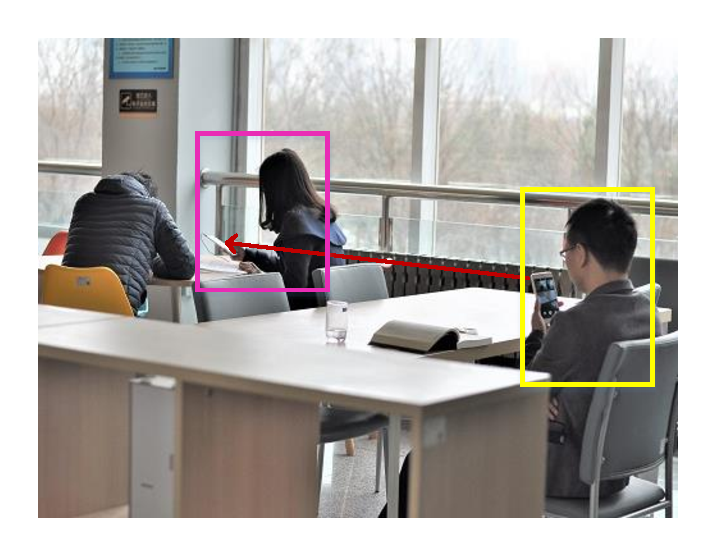
\includegraphics[height=3cm]{fig/1-3.pdf}\\
             \footnotesize (c) The video was recorded from a distance of 2.5 meters.
            \end{minipage}
        }
        \hspace{0.5cm}
        \subfigure{
            \begin{minipage}[t]{3.5cm}
            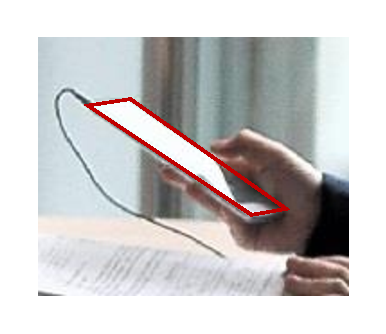
\includegraphics[height=3cm]{fig/1-4.pdf}\\
             \footnotesize (d) The device screen seen from the video filmed in (c).
            \end{minipage}
        }
        \subfigure{
            \begin{minipage}[t]{3.5cm}
            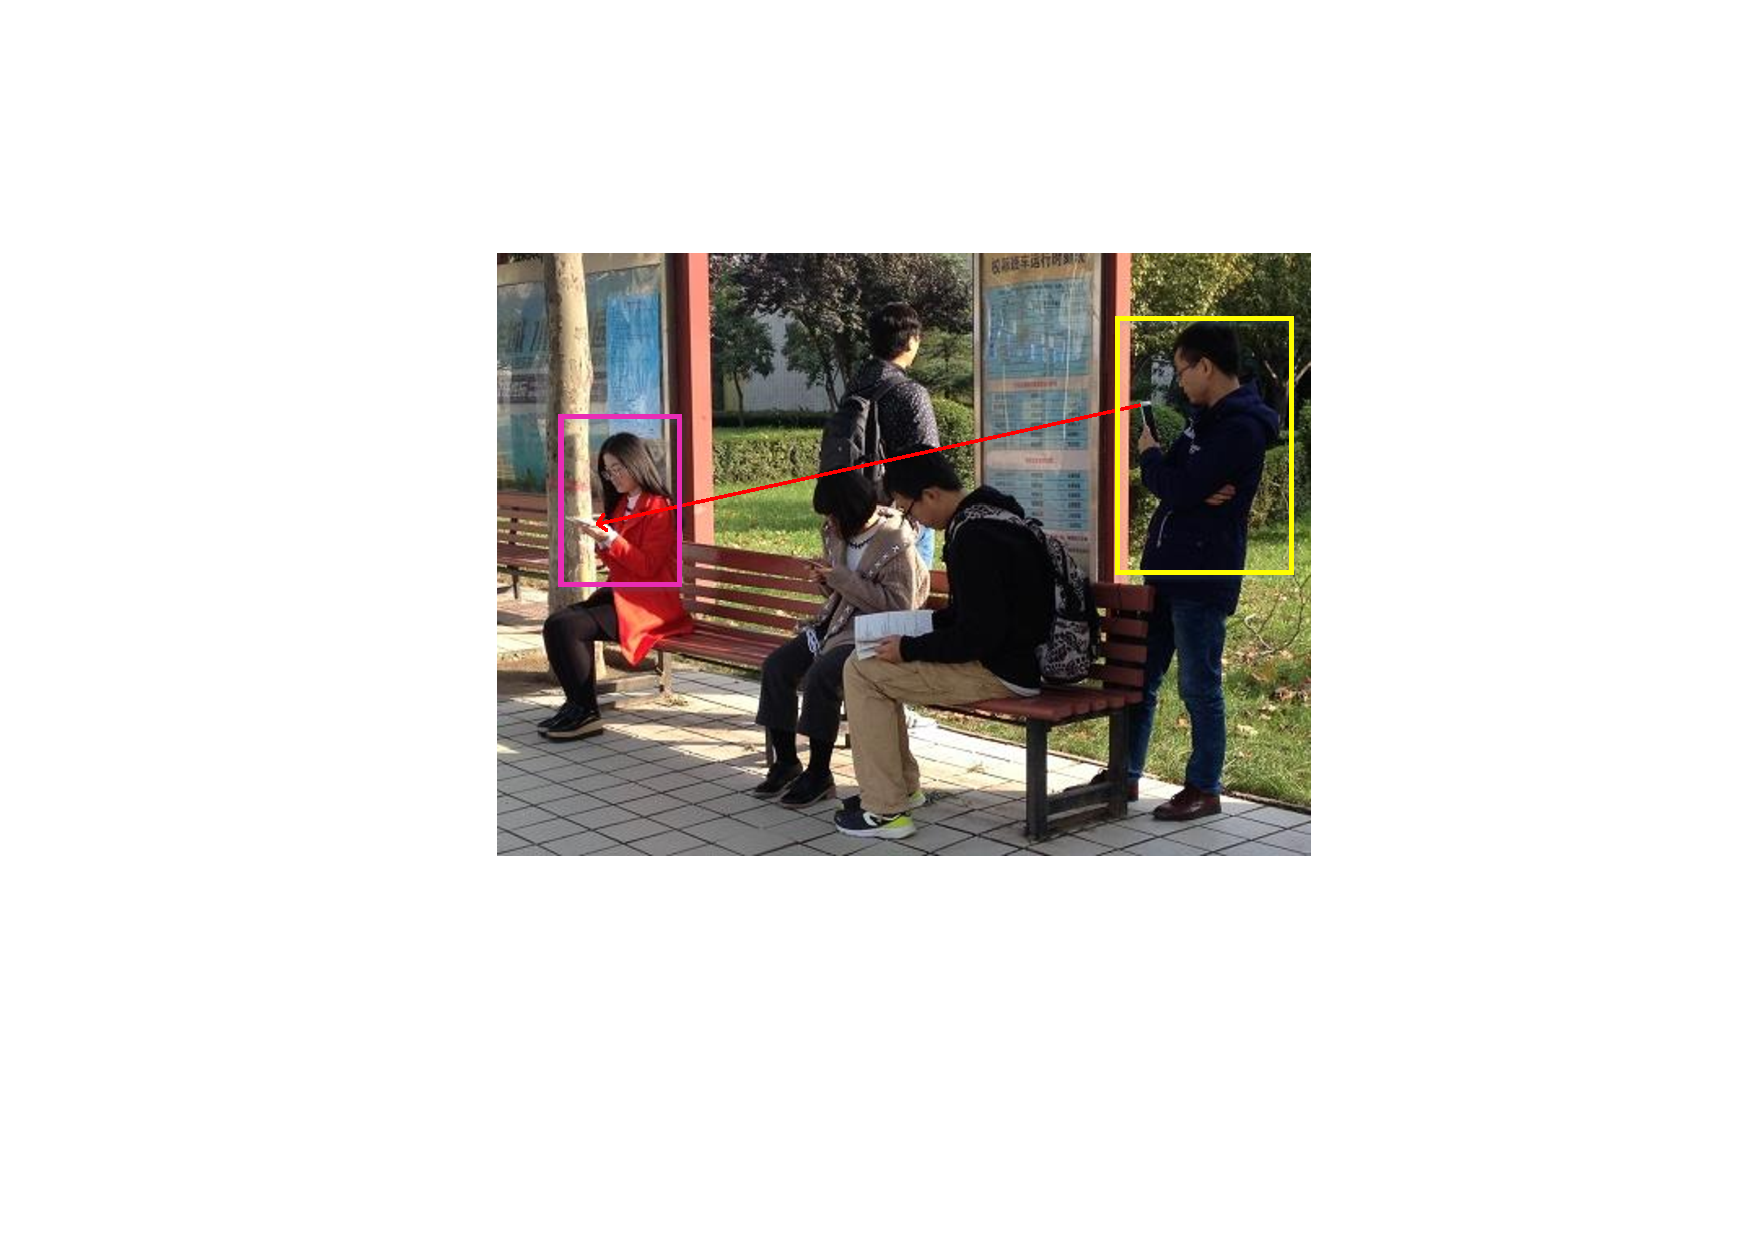
\includegraphics[height=3cm]{fig/1-5.pdf}\\
             \footnotesize (e) An outdoor filming scenario.
             %The user is focusing his attention on searching for learning material in classroom.
            \end{minipage}
        }
        \hspace{0.5cm}
        \subfigure{
            \begin{minipage}[t]{3.5cm}
            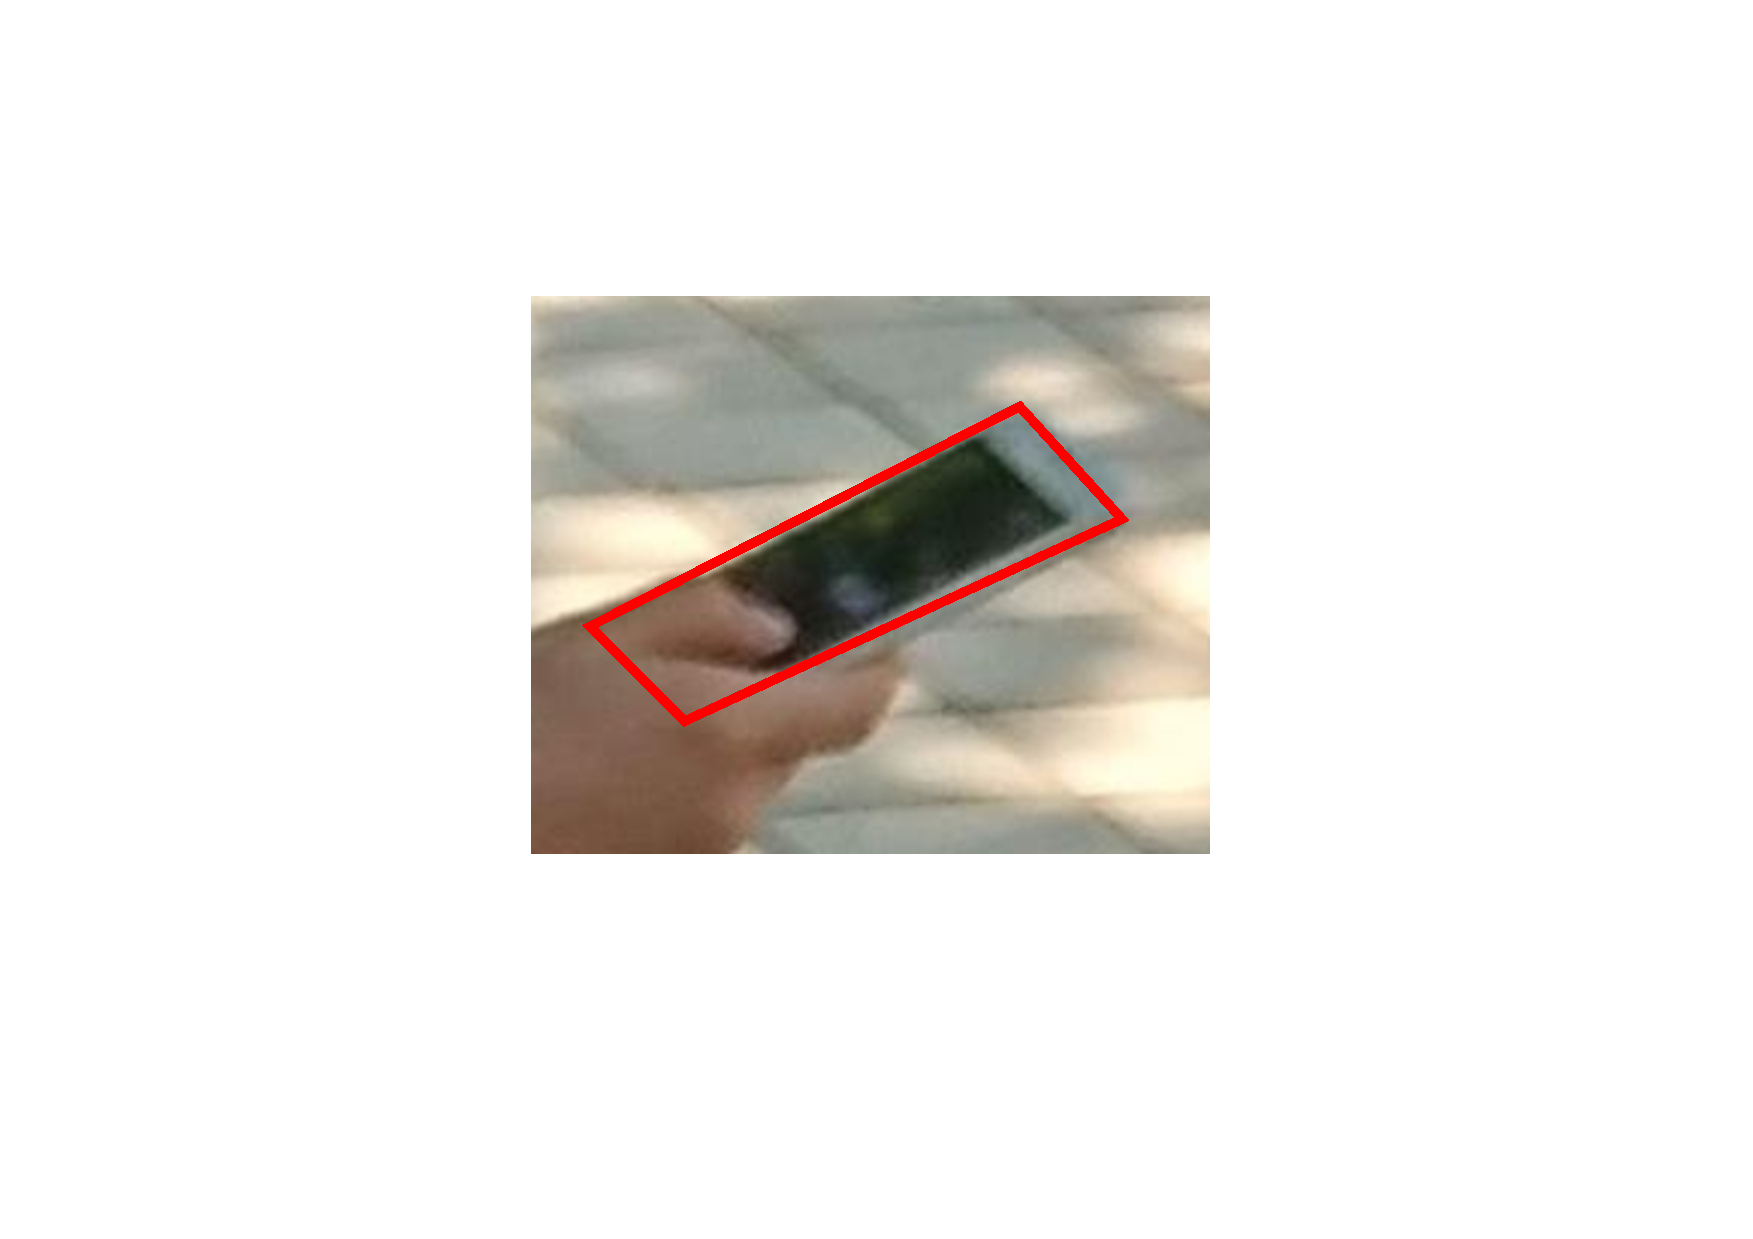
\includegraphics[height=3cm]{fig/1-6.pdf}\\
             \footnotesize (f)
             The device screen seen from the video filmed in (e).
            \end{minipage}
        }
        \vspace{-2mm}
        \caption{Examples of scenarios in which a mobile phone camera is used to film the unlocking process.
        In these scenarios, the camera does not need to have a clear sight of the screen.}
        \label{fig:fig1}
        \vspace{-5mm}
    \end{figure}


We thoroughly evaluate our approach using 120 unique patterns collected from independent users. We show that our approach is effective in inferring candidate patterns and as a result, an attacker can unlock
the target device with a success rate of over 95\% (up to 97.5\%) in five attempts.
We demonstrate that, in contrast to many people's belief, complex patterns do not provide stronger protection over simple patterns under our attack. According to a recent study~\cite{alpnorway}, people tend to use complex
patterns for critical applications such as online banking and shopping applications. 
Our finding suggests that using pattern lock to protect sensitive information could be risky.
\FIXED{Intuitively, our approach is able to crack PIN-based passwords by analyzing the fingertip movement when typing the passwords. We evaluate our approach using 30 4-digital PIN-based passwords and the experimental result shows we can break most of passwords within five attempts.}

\FIXED{Given the wide usage of pattern lock, we propose and implement a prototype of improved pattern lock method. This locking method can effectively defend against video-based attack without external hardware.}

\noindent \textbf{Contributions} This work is the first attack to reconstruct graphical patterns from video footage without requiring the video to capture any contents displayed on the screen.
Our attack exploits techniques developed in the computer vision domain to address the key challenges highlighted above.
The key contribution of this paper is a new attack for Android pattern lock that has not seen in prior work. This paper makes the following specific contributions:

\begin{itemize}
\item \emph{A New Attack.}% This is the first work on exploiting video-based side-channels to attack
%Android pattern lock (Section~\ref{section:overview}).
This is the first work to reconstruct locking patterns without relying on
the content shown on the screen (Section~\ref{sec:scenarios}). %Our approach can accurately
%extract the correct pattern from video footage filmed using a mobile camera that does not directly faces the target device.
Experimental results show that our method can break over
95\% of the lock patterns in five attempts (Section~\ref{sec:overall_rate}). Given that the Android
operating system (OS) allows five tries before
locking the device, our attack represents a real threat for pattern lock.

\item \emph{Identifying New Vulnerabilities.}
According to a recent study~\cite{DBLP:conf/soups/2014}, direct observation techniques, e.g. shoulder surfing, are considered to be a low risk due to the close distance between the attacker and the user (in order to gain a clear sight of the device screen).
As a result, many users may underestimate the dangers from using pattern lock in public places.
Under our attack, filming can be carried out at a distance of 2 meters from the user and the camera does not need to directly face the target device. Such a camera setting makes our attack less likely to raise suspicion and more likely to success when compared to direct observation techniques.
For
instance, the video can be filmed by an adversary who pretends to interact with his phone, sitting next to
the user in a public place (see Figure~\ref{fig:fig1}). In many similar scenarios, users will not be suspicious of the attacker's behavior.

\item \emph{New Findings.} Our study suggests that complex patterns are more vulnerable
under video-based attacks (Section~\ref{sec:overall_rate}). This finding debunks many people's conception
that more complex patterns give stronger protection. Therefore, our work sheds new insights on
 the practical use of pattern lock.

\end{itemize}
